\documentclass[11pt]{article}
% This is Marcus's style file, for little research notes and so on.  I
% keep this in $HOME/texmf/tex/latex, because kpsewhich
% -var-value=TEXMFHOME tells me that ($HOME/texmf) is where latex
% looks, at least under Ubuntu 12.10

\renewcommand{\familydefault}{\sfdefault} % use sans serif fonts
\usepackage{graphicx}
\usepackage[usenames]{color} % so you can {\color{red} anything}, etc.
\usepackage[fleqn]{amsmath}
\usepackage{amsmath}
\usepackage{amssymb,amsfonts}
\setlength{\textwidth}{16cm}
\setlength{\textheight}{24cm}
\hoffset=-2cm
\voffset=-2cm
\raggedbottom
\setlength{\parindent}{0in}
\setlength{\parskip}{0.14in plus 0.07in minus 0.07in}

\setcounter{tocdepth}{2} % determines the depth to which tableofcontents goes

%--------------------------------
\newcommand{\Line}[0]{\rule{0cm}{0cm}\\\hrule\rule{0cm}{0cm}}
\newcommand{\independent}{\protect\mathpalette{\protect\independenT}{\perp}}
\def\independenT#1#2{\mathrel{\rlap{$#1#2$}\mkern2mu{#1#2}}}
\newcommand{\dependent}{\not\independent}
\newcommand{\data}{\mathcal{D}}
\newcommand{\scriptL}{\mathcal{L}}
\newcommand{\mat}[1]{\ensuremath{\mathbf{#1}}} % vectors/matrices, x,A,B etc.
\newcommand{\gmat}[1]{\mbox{\boldmath${#1}$}}  % vectors/matrices Greek symbols
\newcommand{\swrt}[2]{\frac{\partial #1}{\partial #2}} % partial derivative of single symbol
\newcommand{\bwrt}[1]{\frac{\partial}{\partial #1}} % partial derivative of something big
\newcommand{\bA}{\mat{A}}
\newcommand{\bh}{\mat{h}}
\newcommand{\bw}{\mat{w}}
\newcommand{\bv}{\mat{v}}
\newcommand{\bx}{\mat{x}}
\newcommand{\by}{\mat{y}}
\newcommand{\bz}{\mat{z}}
\newcommand{\bp}{\mat{p}}
\newcommand{\br}{\mat{r}}
\newcommand{\bs}{\mat{s}}
\newcommand{\bt}{\mat{t}}
\newcommand{\bu}{\mat{u}}
\newcommand{\bm}{\mat{m}}
\newcommand{\bn}{\mat{n}}
\newcommand{\bc}{\mat{c}}
\newcommand{\bC}{\mat{C}}
\newcommand{\bH}{\mat{H}}
\newcommand{\bM}{\mat{M}}
\newcommand{\bT}{\mat{T}}
\newcommand{\bW}{\mat{W}}
\newcommand{\bX}{\mat{X}}
\newcommand{\bY}{\mat{Y}}
\newcommand{\bZ}{\mat{Z}}
\newcommand{\balpha}{\mat{\alpha}}
\newcommand{\bSigma}{\mat{\Sigma}}
\newcommand{\btheta}{\mathbf{\theta}}
\newcommand{\wo}{\mat{\backslash}}
\newcommand{\bCinv}{\mat{C}^{-1}}
\newcommand{\bCinvPrime}{\mat{C^\prime}^{-1}}
\newcommand{\bkNN}{\mat{k}}
\newcommand{\T}{\ensuremath{\textit{T}}}
\newcommand{\Dir}{\ensuremath{\text{Dir}}}

\newcommand{\Bel}[0]{\text{Bel}}
\newcommand{\on}[0]{\text{on}}
\newcommand{\off}[0]{\text{off}}
\newcommand{\ith}[0]{\text{$i^\text{th}\;$}}
\newcommand{\jth}[0]{\text{$j^\text{th}\;$}}
\newcommand{\kth}[0]{\text{$k^\text{th}\;$}}
\newcommand{\wth}[0]{\text{$w^\text{th}\;$}}
\newcommand{\dth}[0]{\text{$d^\text{th}\;$}}
\newcommand{\nth}[0]{\text{$n^\text{th}\;$}}
\newcommand{\tth}[0]{\text{$t^\text{th}\;$}}

\newcommand{\half}[0]{\text{\tiny$\frac{1}{2}$}}
\newcommand{\onethird}[0]{\text{\tiny$\frac{1}{3}$}}
\newcommand{\twothirds}[0]{\text{\tiny$\frac{2}{3}$}}

\newcommand{\real}{\mathbb{R}}
\newcommand{\reals}{\mathbb{R}}
\newcommand{\Expectation}{\mathbb{E}}
\newcommand{\expectation}{\mathbb{E}}
\newcommand{\obs}{\mathrm{obs}}
\newcommand{\tinyhalf}{\mbox{\tiny $\frac{1}{2}$}}

\newcommand{\tick}{\ding{51}}
\newcommand{\btick}{\ding{52}}
\newcommand{\cross}{\ding{55}}
\newcommand{\bcross}{\ding{56}}

  

\title{self-aware by 2020, or bust}
\author{frean, hogg}
\begin{document}
\maketitle

%\tableofcontents

\section{old stuff: Bayesian model comparison for locating sources}

An image (and its sub-images) can be modelled as a distribution over
pixel intensities. Radio astronomy images can be thought of as
primarily background with an unknown number of spatially extended
sources; and so these images can be thought of as a mixture of
``background" and ``source" distributions. Continuous pixel intensity
values in astronomical images can be discretised by ``binning" them
over $K$ pixel intensity ranges. These bins needn't necessarily be
equally spaced over the pixel intensity range, but may be constructed
using a different strategy, for example bins that are distributed
across the pixel intensity range so that there is equal occupancy in
each bin\footnote{Better still, use the Frean/Friedlander Dirichlet bins scheme. OR better better still still, use the mean of a {\it bunch of likelihoods} each calculated using a different sample for the bin borders. That'd be the best I reckon.}.

Rather than modelling an image as a mixture of two fixed multinomial
distributions; we might want to incorporate the variablity of the
background and source distributions into our model and therefore
use Dirichlet distributions as our background and source
distributions. For any particular sub-image fixed background and
source multinomial distributions can be drawn from their respective
Dirichlet distributions.

Dir Mult distribution is... what it is.  Has hyperparameters
$\alpha_{1..K}$. For some vector of counts $\bn$ in $K$ bins of a histogram,
integrating out the multinomial distributions that result from the
Dirichlets gives the likelihood:
\begin{align}
P(\bn|\alpha) &= \frac{\Gamma(A)}{\Gamma(N+A)} \prod_k \frac{\Gamma(\bn_k+\alpha_k)}{\Gamma(\alpha_k)}  
\label{eq:muldir} 
\intertext{where}
A &= \sum_k \alpha_k, \;\;\;\;\;\;\;\; N = \sum_k \bn_k
\end{align}
Taking logs,
\begin{align}
\log P(\bn|\alpha) &= \log \Gamma(A) - \log \Gamma(N+A) + \sum_k \log \Gamma(\bn_k+\alpha_k) - \log \Gamma(\alpha_k) \label{eq:logmultdir}
\end{align}
so the marginal likelihood is very easy to evaluate.

Given that the number of background pixels in such an image far
outnumber the source pixels, and that the variability among background
pixels is lower than that for source pixels, we might expect the
$\alpha^B$ vector for the background distribution $B$ to be large and
relatively uniform, when compared to the $\alpha^S$ vector for the
source distribution $S$, which contains much smaller values. 

[nb. This is a model which explicitly does {\it not} model sources, in
the usual sense. Saints Osho and Krishnamurti would surely approve of
the backwards-ness of this.]

The Frean {\it et.al.} maxent paper found Bayes factor, namely the
ratio of posterior probabilities under two models, one of which was
very well specified (the background) and one completely unspecified
(sources). Moving and aligning the region so as to maximize this in
favour of the source model amounts to a source finding algorithm. That
is, we maximize
\begin{align}
\text{DMRatio} &= \log \frac{P(\alpha^S | \bn)}{P(\alpha^B | \bn)} \label{eq:score} \\
&= \log \frac{P(\bn | \alpha^S)}{P(\bn | \alpha^B)} \;\; + \; \log \frac{P(\alpha^S)}{P(\alpha^B)}
\end{align}
We can think of this as a mixture with two components then, with the
hyperparameters of both being specified {\it a priori}.

\section{new thought}
For a given region in an image, consider a mixture of (say) $K$
components, where each component is a Dirichlet-multinomial
distribution parameterised by $\boldsymbol{\alpha}_k$.  Picture of the
PGM in fig \ref{fig:mixDirMults}.

\begin{figure}[htb]
\begin{center}
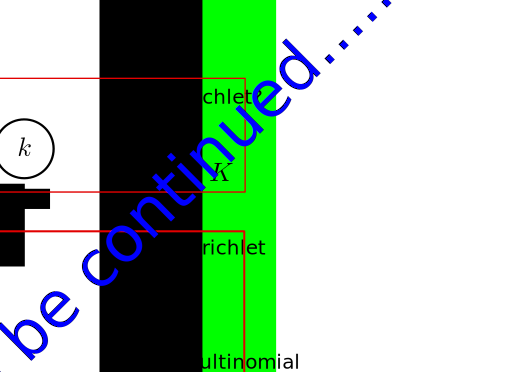
\includegraphics[width=.5\textwidth]{./pics/mix_of_DirMults}
\end{center}
\caption{\label{fig:mixDirMults}
incomplete
}
\end{figure}

But couldn't we learn them instead, in a form of EM?

ANd couldn't we have more than 2?

Start with 2 and go to 3? and so on?

What are the possibilities? 

That's what I think the project is......


\end{document}
